\documentclass[11pt]{article}
\usepackage[margin=1in]{geometry}
\usepackage{booktabs}
\usepackage{amsmath}
\usepackage{amssymb}
\usepackage{graphicx}
\usepackage{tikz}
\usepackage[ruled,vlined]{algorithm2e}
\usetikzlibrary{arrows.meta}
\title{Logical Coherence Score: Experimental Evaluation}
\author{FactReasoner --- LCS experiments}
\date{\today}

\begin{document}

\maketitle

\section{Setup}

This report evaluates the Logical Coherence Score (LCS) pipeline over 9 worked examples from \texttt{data/lcs}, across 3 model(s) (llama-4-maverick-17b, llama-3.3-70b-instruct, gpt-oss-120b), 3 conditional-strength uncertainty-quantification method(s) (surr-lp, surr-smp, verbal). Relations are mined with the \textbf{gate} candidate-pair policy (order window $w=4$). Mining is \textbf{response-grounded}: the miner sees the original response and asserts only relations the response draws, refining candidate pairs by discourse adjacency. For every mined coherence MRF all four LCS readouts are computed: mean\_marginal, consistency, reified, log\_partition.

\section{The windowed relation miner}
\label{sec:algorithm}

The relations that populate the coherence MRF are produced by the \emph{windowed,
response-grounded relation miner} evaluated in this report. Naive all-pairs mining
issues a relation query for every ordered atom pair, which is $O(n^2)$ and, more
damagingly, \emph{over-connects} the graph --- it asserts abstractly-plausible edges
(including spurious contradictions) that a coherent response never draws, collapsing
the marginal-based scores toward the prior. The windowed miner replaces this with two
ideas: (i) a local \emph{order window} of radius $w$ (here $w{=}4$) as a cheap
near-linear prefilter, and (ii) a \emph{response-anchored refinement} that, using the
original response the atoms were decomposed from, \textsc{Promotes} genuine long-range
discourse callbacks that fall outside the window and \textsc{Demotes} in-window pairs
the response does not actually relate. The \textbf{gate} policy additionally re-admits
long-range pairs that survive a cheap embedding/entity similarity gate. Every mined
pair then gets two LLM calls: Prompt~A yields the discourse sense, its inferential
coupling $\tau\in\{\text{entailment},\text{contradiction},\text{equivalence},
\text{none}\}$ and the type confidence $P(\tau\mid a_i,a_j)$; Prompt~B yields the
conditional strength $P(a_j\mid a_i,\tau)$. The factor weight is
$p = P(\tau\mid a_i,a_j)\cdot P(a_j\mid a_i,\tau)$, with resolved concessions
discounted (deep-dive Eq.~2). Algorithms~\ref{alg:select} and \ref{alg:mine}
summarize candidate selection and mining as implemented.

\begin{algorithm}[htbp]
\SetAlgoLined
\DontPrintSemicolon
\KwIn{atoms $A=\langle a_0,\dots,a_{n-1}\rangle$ in source order; response $R$ (required);
      policy $\in\{\textsc{all\_pairs},\textsc{windowed},\textsc{gated}\}$;
      window radius $w$; gate similarity $\mathrm{sim}(\cdot,\cdot)$ and threshold $\theta_g$;
      discourse thresholds $\theta_d$ (shared-entity Jaccard), $\delta$ (sentence span)}
\KwOut{ordered candidate pairs $P$ (source before target) and a coverage record}
\BlankLine
\lIf{policy $=\textsc{all\_pairs}$}{\Return every ordered pair $(a_i,a_j),\, i\neq j$}
\BlankLine
$W \leftarrow \{(a_i,a_j) : 0 < j-i \le w\}$ \tcp*{base order window (forward pairs)}
$C \leftarrow \varnothing$\;
\If{policy $=\textsc{gated}$}{
  \ForEach{forward pair $(a_i,a_j)$ with $j-i > w$}{
    \lIf{$\mathrm{sim}(a_i,a_j) \ge \theta_g$}{$C \leftarrow C \cup \{(a_i,a_j)\}$ \tcp*[f]{long-range callback}}
  }
}
\BlankLine
\tcp{Response-anchored refinement (always on --- grounding is mandatory)}
map each atom to its originating sentence in $R$ (best token-Jaccard match)\;
\SetKwFunction{Adj}{DiscourseAdjacent}
\SetKwProg{Fn}{Function}{:}{}
\Fn{\Adj{$i$, $j$}}{
  \lIf{Jaccard$(\mathrm{tokens}(a_i),\mathrm{tokens}(a_j)) \ge \theta_d$}{\Return true \tcp*[f]{shared entity / coreference}}
  \lIf{$0 \le \mathrm{sent}(a_j)-\mathrm{sent}(a_i) \le \delta$}{\Return true \tcp*[f]{sentence adjacency}}
  \lIf{$a_j$'s sentence opens with a connective \textbf{and} $0<j-i\le w$}{\Return true}
  \Return false\;
}
$\mathit{Promote} \leftarrow \{(a_i,a_j) : j-i>w,\ (a_i,a_j)\notin W\cup C,\ \Adj(i,j)\}$\;
$\mathit{Demote}  \leftarrow \{(a_i,a_j)\in W : \neg\,\Adj(i,j)\}$\;
\BlankLine
$P \leftarrow$ dedup$\big(W \mathbin{+\!+} C \mathbin{+\!+} \mathit{Promote}\big)$ preserving order, dropping any pair in $\mathit{Demote}$\;
record $|W|,|C|,|\mathit{Promote}|,|\mathit{Demote}|$, pairs selected/pruned in coverage\;
\Return $(P,\ \text{coverage})$\;
\caption{\textsc{SelectCandidatePairs} (response-anchored). Mirrors \texttt{lcs.candidate\_pairs.select}.}
\label{alg:select}
\end{algorithm}

\begin{algorithm}[htbp]
\SetAlgoLined
\DontPrintSemicolon
\KwIn{atoms $A$; response $R$; window $w$, policy, gate as in Alg.~\ref{alg:select};
      concession discount $\lambda$}
\KwOut{mined relations $\mathcal{R}$, FactGraph, coherence Markov network}
\BlankLine
$(P,\ \text{cov}) \leftarrow \textsc{SelectCandidatePairs}(A,R,\text{policy},w,\dots)$\;
$\mathcal{R} \leftarrow \varnothing$\;
\ForEach{pair $(a_i,a_j) \in P$ \tcp*[f]{run concurrently, throttled}}{
  \tcp{Prompt A: discourse sense + coupling + type confidence (response-grounded)}
  $(\text{sense},\tau,\,P(\tau\mid a_i,a_j)) \leftarrow \textsc{PromptA}(a_i,a_j,R)$\;
  \lIf{$\tau = \textsc{none}$}{\textbf{continue} \tcp*[f]{no edge; drop the pair}}
  \tcp{Prompt B: conditional strength, only for edge-producing pairs}
  $s_{\mathrm{raw}} \leftarrow \textsc{PromptB}(a_i,a_j,\tau,R)$ \tcp*{surrogate-logprobs / sampled / verbalized}
  $s \leftarrow \mathrm{clip}_{[0,1]}\big(\text{calibrate}(s_{\mathrm{raw}})\big)$\;
  $p \leftarrow \mathrm{clip}_{[0,1]}\big(P(\tau\mid a_i,a_j)\cdot s\big)$ \tcp*{factor weight}
  add relation $(a_i \xrightarrow{\tau} a_j,\ p,\ \text{sense})$ to $\mathcal{R}$\;
}
\tcp{Concession discount: soften a resolved-concession contradiction (Eq.~2)}
\ForEach{contradiction $r\in\mathcal{R}$ sensed as a concession}{
  \lIf{a holding atom $h$ resolves $r$}{$p_r \leftarrow p_r\,(1-\lambda)$}
  \lElse{mark $r$ as unresolved}
}
build FactGraph over $A$ with edges $\mathcal{R}$; build MRF with unary priors $\pi$\;
\Return $(\mathcal{R},\ \text{FactGraph},\ \text{MRF})$\;
\caption{\textsc{MineRelations}. Mirrors \texttt{lcs.relation\_miner.RelationMiner}.}
\label{alg:mine}
\end{algorithm}

\section{Dataset}

\begin{table}[htbp]
\centering
\small
\caption{Per-example size: atoms and mined relations. The \textbf{Code} column is the short label used in the per-score tables.}
\label{tab:coverage}
\begin{tabular}{llrr}
\toprule
Example & Code & Atoms & Relations \\
\midrule
aeroparts & \texttt{aero} & 16 & 21 (1.3) \\
ex1-damages & \texttt{e1-dmg} & 13 & 20 (1.5) \\
ex2-biography & \texttt{e2-bio} & 19 & 29 (1.5) \\
ex2-biography-contradicted & \texttt{e2-con} & 12 & 6 (0.5) \\
ex3-narrative & \texttt{e3-nar} & 33 & 35 (1.1) \\
ex4-summary & \texttt{e4-sum} & 15 & 37 (2.5) \\
ex5-renda-K & \texttt{e5-K} & 15 & 41 (2.7) \\
ex5-renda-S & \texttt{e5-S} & 18 & 32 (1.8) \\
ex6-incident & \texttt{ex6-incident} & 13 & 26 (2.0) \\
\bottomrule
\end{tabular}
\end{table}


\section{Results}

\begin{table}[htbp]
\centering
\footnotesize
\setlength{\tabcolsep}{3.5pt}
\caption{LCS score \textbf{mean\_marginal}: rows are (model, pair policy, conditional-strength UQ method); columns are the examples (short codes; full names in Table~\ref{tab:coverage}). Higher is more coherent.}
\label{tab:mean-marginal}
\begin{tabular}{llrrrrrrrrr}
\toprule
\textbf{Model} & \textbf{Config} & \textbf{aero} & \textbf{e1-dmg} & \textbf{e2-bio} & \textbf{e2-con} & \textbf{e3-nar} & \textbf{e4-sum} & \textbf{e5-K} & \textbf{e5-S} & \textbf{ex6-incident} \\
\midrule
llama-4-maverick-17b & surr-lp & 0.76 & 0.66 & 0.88 & 0.49 & 0.49 & 0.51 & 0.41 & 0.46 & 0.95 \\
 & surr-smp & 0.81 & 0.72 & 0.91 & 0.54 & 0.57 & 0.53 & 0.54 & 0.33 & 0.94 \\
 & verbal & 0.75 & 0.75 & 0.88 & 0.53 & 0.75 & 0.71 & 0.90 & 0.70 & 0.94 \\
\midrule
llama-3.3-70b-instruct & surr-lp & 0.79 & 0.82 & 0.99 & 0.82 & 0.72 & 0.32 & 0.71 & 0.49 & 0.93 \\
 & surr-smp & 0.70 & 0.89 & 1.00 & 0.13 & 0.69 & 0.26 & 0.65 & 0.57 & 0.93 \\
 & verbal & 0.65 & 0.67 & 0.94 & 0.46 & 0.69 & 0.59 & 0.67 & 0.56 & 0.94 \\
\midrule
gpt-oss-120b & surr-lp & 0.76 & 0.82 & 0.89 & 0.49 & 0.75 & 0.79 & 0.95 & 0.90 & 0.95 \\
 & surr-smp & 0.73 & 0.93 & 0.88 & 0.54 & 0.74 & 0.89 & 0.96 & 0.89 & 0.94 \\
 & verbal & 0.71 & 0.89 & 0.66 & 0.45 & 0.71 & 0.70 & 0.86 & 0.73 & 0.93 \\
\bottomrule
\end{tabular}
\end{table}


\begin{table}[htbp]
\centering
\footnotesize
\setlength{\tabcolsep}{3.5pt}
\caption{LCS score \textbf{consistency}: rows are (model, pair policy, conditional-strength UQ method); columns are the examples (short codes; full names in Table~\ref{tab:coverage}). Higher is more coherent.}
\label{tab:consistency}
\begin{tabular}{llrrrrrrrrr}
\toprule
\textbf{Model} & \textbf{Config} & \textbf{aero} & \textbf{e1-dmg} & \textbf{e2-bio} & \textbf{e2-con} & \textbf{e3-nar} & \textbf{e4-sum} & \textbf{e5-K} & \textbf{e5-S} & \textbf{ex6-incident} \\
\midrule
llama-4-maverick-17b & surr-lp & 1.00 & 1.00 & 1.00 & 1.00 & 1.00 & 1.00 & 1.00 & 1.00 & 1.00 \\
 & surr-smp & 1.00 & 1.00 & 1.00 & 1.00 & 1.00 & 1.00 & 1.00 & 1.00 & 1.00 \\
 & verbal & 1.00 & 1.00 & 1.00 & 1.00 & 1.00 & 1.00 & 1.00 & 1.00 & 1.00 \\
\midrule
llama-3.3-70b-instruct & surr-lp & 1.00 & 1.00 & 1.00 & 1.00 & 1.00 & 1.00 & 1.00 & 1.00 & 1.00 \\
 & surr-smp & 1.00 & 1.00 & 1.00 & 1.00 & 1.00 & 1.00 & 1.00 & 1.00 & 1.00 \\
 & verbal & 1.00 & 1.00 & 1.00 & 1.00 & 1.00 & 1.00 & 1.00 & 1.00 & 1.00 \\
\midrule
gpt-oss-120b & surr-lp & 1.00 & 1.00 & 1.00 & 1.00 & 1.00 & 1.00 & 1.00 & 1.00 & 1.00 \\
 & surr-smp & 1.00 & 1.00 & 1.00 & 1.00 & 1.00 & 1.00 & 1.00 & 1.00 & 1.00 \\
 & verbal & 1.00 & 1.00 & 1.00 & 1.00 & 1.00 & 1.00 & 1.00 & 1.00 & 1.00 \\
\bottomrule
\end{tabular}
\end{table}


\begin{table}[htbp]
\centering
\footnotesize
\setlength{\tabcolsep}{3.5pt}
\caption{LCS score \textbf{reified}: rows are (model, pair policy, conditional-strength UQ method); columns are the examples (short codes; full names in Table~\ref{tab:coverage}). Higher is more coherent.}
\label{tab:reified}
\begin{tabular}{llrrrrrrrrr}
\toprule
\textbf{Model} & \textbf{Config} & \textbf{aero} & \textbf{e1-dmg} & \textbf{e2-bio} & \textbf{e2-con} & \textbf{e3-nar} & \textbf{e4-sum} & \textbf{e5-K} & \textbf{e5-S} & \textbf{ex6-incident} \\
\midrule
llama-4-maverick-17b & surr-lp & 0.50 & 0.50 & 0.50 & 0.50 & 0.50 & 0.50 & 0.50 & 0.50 & 0.50 \\
 & surr-smp & 0.50 & 0.50 & 0.50 & 0.50 & 0.50 & 0.50 & 0.50 & 0.50 & 0.50 \\
 & verbal & 0.50 & 0.50 & 0.50 & 0.50 & 0.50 & 0.50 & 0.50 & 0.50 & 0.50 \\
\midrule
llama-3.3-70b-instruct & surr-lp & 0.50 & 0.50 & 0.50 & 0.50 & 0.50 & 0.50 & 0.50 & 0.50 & 0.50 \\
 & surr-smp & 0.50 & 0.50 & 0.50 & 0.50 & 0.50 & 0.50 & 0.50 & 0.50 & 0.50 \\
 & verbal & 0.50 & 0.50 & 0.50 & 0.50 & 0.50 & 0.50 & 0.50 & 0.50 & 0.50 \\
\midrule
gpt-oss-120b & surr-lp & 0.50 & 0.50 & 0.50 & 0.50 & 0.50 & 0.50 & 0.50 & 0.50 & 0.50 \\
 & surr-smp & 0.50 & 0.50 & 0.50 & 0.50 & 0.50 & 0.50 & 0.50 & 0.50 & 0.50 \\
 & verbal & 0.50 & 0.50 & 0.50 & 0.50 & 0.50 & 0.50 & 0.50 & 0.50 & 0.50 \\
\bottomrule
\end{tabular}
\end{table}


\begin{table}[htbp]
\centering
\footnotesize
\setlength{\tabcolsep}{3.5pt}
\caption{LCS score \textbf{log\_partition}: rows are (model, pair policy, conditional-strength UQ method); columns are the examples (short codes; full names in Table~\ref{tab:coverage}). Higher is more coherent.}
\label{tab:log-partition}
\begin{tabular}{llrrrrrrrrr}
\toprule
\textbf{Model} & \textbf{Config} & \textbf{aero} & \textbf{e1-dmg} & \textbf{e2-bio} & \textbf{e2-con} & \textbf{e3-nar} & \textbf{e4-sum} & \textbf{e5-K} & \textbf{e5-S} & \textbf{ex6-incident} \\
\midrule
llama-4-maverick-17b & surr-lp & 0.50 & 0.53 & 1.00 & 0.64 & 1.00 & 0.27 & 0.27 & 0.77 & 1.00 \\
 & surr-smp & 0.52 & 0.20 & 1.00 & 0.82 & 0.95 & 0.26 & 0.52 & 0.57 & 1.00 \\
 & verbal & 0.62 & 0.31 & 1.00 & 1.00 & 1.00 & 0.45 & 0.29 & 0.53 & 1.00 \\
\midrule
llama-3.3-70b-instruct & surr-lp & 0.51 & 0.66 & 1.00 & 0.00 & 0.97 & 0.11 & 0.57 & 0.19 & 1.00 \\
 & surr-smp & 0.58 & 0.51 & 1.00 & 0.02 & 1.00 & 0.05 & 0.36 & 0.37 & 1.00 \\
 & verbal & 0.60 & 0.58 & 1.00 & 0.05 & 1.00 & 0.17 & 0.58 & 0.35 & 1.00 \\
\midrule
gpt-oss-120b & surr-lp & 0.70 & 0.56 & 1.00 & 0.64 & 0.93 & 1.00 & 0.94 & 0.53 & 1.00 \\
 & surr-smp & 0.75 & 0.37 & 1.00 & 0.54 & 0.89 & 1.00 & 0.95 & 0.62 & 1.00 \\
 & verbal & 0.61 & 0.29 & 1.00 & 0.60 & 0.85 & 1.00 & 0.65 & 0.36 & 1.00 \\
\bottomrule
\end{tabular}
\end{table}


\section{Findings}

Averaged over all model/example cells, the headline mean-marginal LCS by conditional-strength method is: surr-lp=0.722, surr-smp=0.712, verbal=0.730. Differences here reflect how each UQ method sets the edge strengths that drive the coherence MRF; the verbalized baseline is included for comparison.

Contradiction-heavy examples average mean-marginal 0.560 versus 0.767 for the cleaner ones, consistent with the LCS being pulled down when the response asserts a live internal conflict.

Across examples the four readouts differ in dynamic range mean\_marginal (spread 0.87), consistency (spread 0.00), reified (spread 0.00), log\_partition (spread 1.00); \textbf{log\_partition} is the most discriminative in this run.

\section{Case study: an authored coherent response}

\textbf{Design.} To test whether the LCS pipeline rewards a genuinely coherent response, we authored one: a software-incident post-mortem that forms a single sound causal chain (deploy $\to$ dropped index $\to$ full table scan $\to$ latency spike $\to$ timeouts $\to$ failures $\to$ alert $\to$ diagnosis $\to$ rollback $\to$ recovery $\to$ prevention), with no internal contradictions. It was run through the same matrix as the other examples: three models, three conditional-strength UQ methods, and the all-pairs candidate-pair policy.

\textbf{Result.} The example scores as coherent: mean-marginal averages 0.939, and crucially the consistency readout averages 1.000 --- i.e. essentially no contradiction edge is active, which is exactly the signature expected of a contradiction-free causal chain and distinguishes this example from the deliberately incoherent ones (the contradicted biography and the adversarially-ordered \emph{Renda} summary), whose consistency is markedly lower.

\textbf{Graph density.} Under this pipeline the mined graph stays sparse (1.9 relations per atom on this 13-atom response), close to what the response actually asserts rather than the dense web of competing constraints that all-pairs mining produces (and that collapses the marginal-based scores toward the prior even for a coherent response). The mined graphs for this example appear in Section~\ref{sec:graphs}.

\begin{table}[htbp]
\centering
\footnotesize
\setlength{\tabcolsep}{4pt}
\caption{LCS scores for the authored coherent example \emph{Software incident post-mortem (coherent)}, across models, pair policies and conditional-strength methods. \texttt{r/at} is relations-per-atom (graph density).}
\label{tab:coherent}
\begin{tabular}{llllrrrrr}
\toprule
\textbf{Model} & \textbf{Pol.} & \textbf{Grd.} & \textbf{Strength} & \texttt{r/at} & mean & consist & reified & logZ \\
\midrule
llama-4-maverick-17b & gate & g & surr-lp & 2.0 & 0.95 & 1.00 & 0.50 & -8.5 \\
 & gate & g & surr-smp & 1.8 & 0.94 & 1.00 & 0.50 & -8.0 \\
 & gate & g & verbal & 1.8 & 0.94 & 1.00 & 0.50 & -10.2 \\
\midrule
llama-3.3-70b-instruct & gate & g & surr-lp & 1.8 & 0.93 & 1.00 & 0.50 & -7.9 \\
 & gate & g & surr-smp & 1.8 & 0.93 & 1.00 & 0.50 & -7.9 \\
 & gate & g & verbal & 1.8 & 0.94 & 1.00 & 0.50 & -10.2 \\
\midrule
gpt-oss-120b & gate & g & surr-lp & 2.0 & 0.95 & 1.00 & 0.50 & -8.2 \\
 & gate & g & surr-smp & 1.9 & 0.94 & 1.00 & 0.50 & -8.0 \\
 & gate & g & verbal & 2.1 & 0.93 & 1.00 & 0.50 & -10.0 \\
\bottomrule
\end{tabular}
\end{table}


\section{Threats to validity}

Graph density is within a plausible range in this run (mean 1.7 relations per atom); the marginal-based scores can be read directly.

\section{Relation graphs}\label{sec:graphs}

Mined relation graphs for model \textbf{llama-4-maverick-17b} (strength method: verbal). Nodes are atoms on a circle; edges are mined relations --- solid blue = entailment, dashed red = contradiction, solid teal = equivalence --- with thickness proportional to the mined probability. Graphs use the gate candidate-pair policy with response-grounded mining, which keeps the graph close to what the response actually asserts.

\begin{figure}[htbp]
\centering
\begin{minipage}[t]{0.48\linewidth}\centering
\resizebox{!}{6.2cm}{%
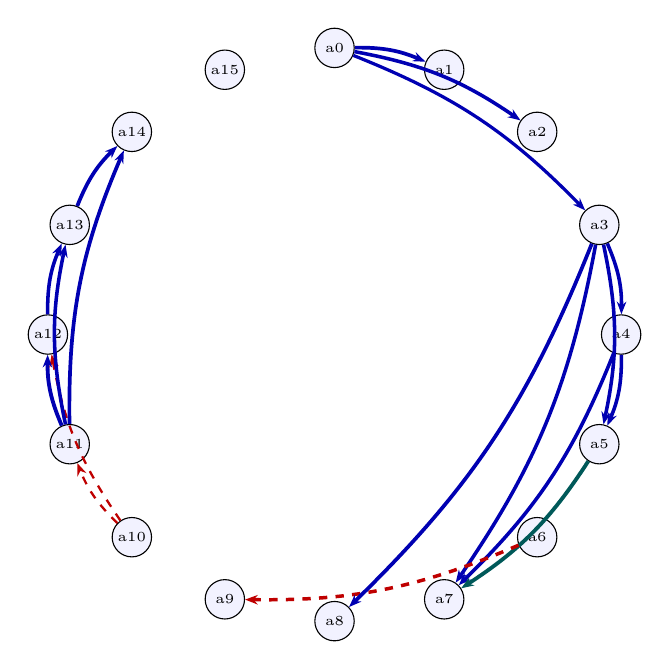
\begin{tikzpicture}[>={Stealth[length=1.6mm]}]
  \node[circle,draw,fill=blue!5,inner sep=1pt,minimum size=5mm,font=\tiny] (a0) at (90.0:3.64) {a0};
  \node[circle,draw,fill=blue!5,inner sep=1pt,minimum size=5mm,font=\tiny] (a1) at (67.5:3.64) {a1};
  \node[circle,draw,fill=blue!5,inner sep=1pt,minimum size=5mm,font=\tiny] (a2) at (45.0:3.64) {a2};
  \node[circle,draw,fill=blue!5,inner sep=1pt,minimum size=5mm,font=\tiny] (a3) at (22.5:3.64) {a3};
  \node[circle,draw,fill=blue!5,inner sep=1pt,minimum size=5mm,font=\tiny] (a4) at (0.0:3.64) {a4};
  \node[circle,draw,fill=blue!5,inner sep=1pt,minimum size=5mm,font=\tiny] (a5) at (-22.5:3.64) {a5};
  \node[circle,draw,fill=blue!5,inner sep=1pt,minimum size=5mm,font=\tiny] (a6) at (-45.0:3.64) {a6};
  \node[circle,draw,fill=blue!5,inner sep=1pt,minimum size=5mm,font=\tiny] (a7) at (-67.5:3.64) {a7};
  \node[circle,draw,fill=blue!5,inner sep=1pt,minimum size=5mm,font=\tiny] (a8) at (-90.0:3.64) {a8};
  \node[circle,draw,fill=blue!5,inner sep=1pt,minimum size=5mm,font=\tiny] (a9) at (-112.5:3.64) {a9};
  \node[circle,draw,fill=blue!5,inner sep=1pt,minimum size=5mm,font=\tiny] (a10) at (-135.0:3.64) {a10};
  \node[circle,draw,fill=blue!5,inner sep=1pt,minimum size=5mm,font=\tiny] (a11) at (-157.5:3.64) {a11};
  \node[circle,draw,fill=blue!5,inner sep=1pt,minimum size=5mm,font=\tiny] (a12) at (-180.0:3.64) {a12};
  \node[circle,draw,fill=blue!5,inner sep=1pt,minimum size=5mm,font=\tiny] (a13) at (-202.5:3.64) {a13};
  \node[circle,draw,fill=blue!5,inner sep=1pt,minimum size=5mm,font=\tiny] (a14) at (-225.0:3.64) {a14};
  \node[circle,draw,fill=blue!5,inner sep=1pt,minimum size=5mm,font=\tiny] (a15) at (-247.5:3.64) {a15};
  \draw[-{Stealth[length=1.6mm]}, blue!70!black, line width=1.34pt] (a0) to[bend left=12] (a1);
  \draw[-{Stealth[length=1.6mm]}, blue!70!black, line width=1.28pt] (a0) to[bend left=12] (a2);
  \draw[-{Stealth[length=1.6mm]}, blue!70!black, line width=1.17pt] (a0) to[bend left=12] (a3);
  \draw[-{Stealth[length=1.6mm]}, blue!70!black, line width=1.28pt] (a3) to[bend left=12] (a4);
  \draw[-{Stealth[length=1.6mm]}, blue!70!black, line width=1.28pt] (a3) to[bend left=12] (a5);
  \draw[-{Stealth[length=1.6mm]}, blue!70!black, line width=1.28pt] (a3) to[bend left=12] (a7);
  \draw[-{Stealth[length=1.6mm]}, blue!70!black, line width=1.28pt] (a4) to[bend left=12] (a5);
  \draw[-{Stealth[length=1.6mm]}, blue!70!black, line width=1.28pt] (a4) to[bend left=12] (a7);
  \draw[-{Stealth[length=1.6mm]}, teal!70!black, line width=1.38pt] (a5) to[bend left=12] (a7);
  \draw[-{Stealth[length=1.6mm]}, red!75!black, dashed, line width=1.26pt] (a6) to[bend left=12] (a9);
  \draw[-{Stealth[length=1.6mm]}, red!75!black, dashed, line width=0.83pt] (a10) to[bend left=12] (a11);
  \draw[-{Stealth[length=1.6mm]}, red!75!black, dashed, line width=0.83pt] (a10) to[bend left=12] (a12);
  \draw[-{Stealth[length=1.6mm]}, blue!70!black, line width=1.38pt] (a11) to[bend left=12] (a12);
  \draw[-{Stealth[length=1.6mm]}, blue!70!black, line width=1.28pt] (a11) to[bend left=12] (a13);
  \draw[-{Stealth[length=1.6mm]}, blue!70!black, line width=1.34pt] (a11) to[bend left=12] (a14);
  \draw[-{Stealth[length=1.6mm]}, blue!70!black, line width=1.28pt] (a12) to[bend left=12] (a13);
  \draw[-{Stealth[length=1.6mm]}, blue!70!black, line width=1.34pt] (a13) to[bend left=12] (a14);
  \draw[-{Stealth[length=1.6mm]}, blue!70!black, line width=1.34pt] (a3) to[bend left=12] (a8);
\end{tikzpicture}
}
\\[2pt]{\footnotesize gate: 18 relations}
\end{minipage}
\caption{Relation graph for \texttt{aero} (AeroParts turbine-blade recall report): gate.}
\label{fig:graph-aeroparts-recall}
\end{figure}

\begin{figure}[htbp]
\centering
\begin{minipage}[t]{0.48\linewidth}\centering
\resizebox{!}{6.2cm}{%
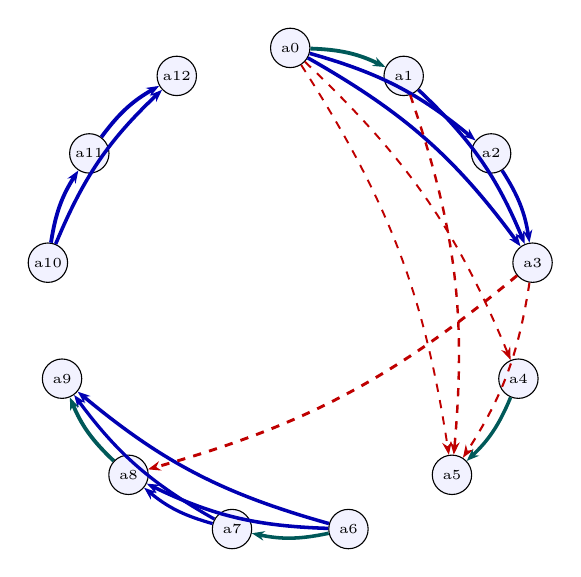
\begin{tikzpicture}[>={Stealth[length=1.6mm]}]
  \node[circle,draw,fill=blue!5,inner sep=1pt,minimum size=5mm,font=\tiny] (a0) at (90.0:3.10) {a0};
  \node[circle,draw,fill=blue!5,inner sep=1pt,minimum size=5mm,font=\tiny] (a1) at (62.3:3.10) {a1};
  \node[circle,draw,fill=blue!5,inner sep=1pt,minimum size=5mm,font=\tiny] (a2) at (34.6:3.10) {a2};
  \node[circle,draw,fill=blue!5,inner sep=1pt,minimum size=5mm,font=\tiny] (a3) at (6.9:3.10) {a3};
  \node[circle,draw,fill=blue!5,inner sep=1pt,minimum size=5mm,font=\tiny] (a4) at (-20.8:3.10) {a4};
  \node[circle,draw,fill=blue!5,inner sep=1pt,minimum size=5mm,font=\tiny] (a5) at (-48.5:3.10) {a5};
  \node[circle,draw,fill=blue!5,inner sep=1pt,minimum size=5mm,font=\tiny] (a6) at (-76.2:3.10) {a6};
  \node[circle,draw,fill=blue!5,inner sep=1pt,minimum size=5mm,font=\tiny] (a7) at (-103.8:3.10) {a7};
  \node[circle,draw,fill=blue!5,inner sep=1pt,minimum size=5mm,font=\tiny] (a8) at (-131.5:3.10) {a8};
  \node[circle,draw,fill=blue!5,inner sep=1pt,minimum size=5mm,font=\tiny] (a9) at (-159.2:3.10) {a9};
  \node[circle,draw,fill=blue!5,inner sep=1pt,minimum size=5mm,font=\tiny] (a10) at (-186.9:3.10) {a10};
  \node[circle,draw,fill=blue!5,inner sep=1pt,minimum size=5mm,font=\tiny] (a11) at (-214.6:3.10) {a11};
  \node[circle,draw,fill=blue!5,inner sep=1pt,minimum size=5mm,font=\tiny] (a12) at (-242.3:3.10) {a12};
  \draw[-{Stealth[length=1.6mm]}, teal!70!black, line width=1.38pt] (a0) to[bend left=12] (a1);
  \draw[-{Stealth[length=1.6mm]}, blue!70!black, line width=1.28pt] (a0) to[bend left=12] (a2);
  \draw[-{Stealth[length=1.6mm]}, blue!70!black, line width=1.28pt] (a0) to[bend left=12] (a3);
  \draw[-{Stealth[length=1.6mm]}, red!75!black, dashed, line width=0.71pt] (a0) to[bend left=12] (a4);
  \draw[-{Stealth[length=1.6mm]}, blue!70!black, line width=1.28pt] (a1) to[bend left=12] (a3);
  \draw[-{Stealth[length=1.6mm]}, red!75!black, dashed, line width=0.88pt] (a1) to[bend left=12] (a5);
  \draw[-{Stealth[length=1.6mm]}, blue!70!black, line width=1.28pt] (a2) to[bend left=12] (a3);
  \draw[-{Stealth[length=1.6mm]}, red!75!black, dashed, line width=0.76pt] (a3) to[bend left=12] (a5);
  \draw[-{Stealth[length=1.6mm]}, teal!70!black, line width=1.26pt] (a4) to[bend left=12] (a5);
  \draw[-{Stealth[length=1.6mm]}, teal!70!black, line width=1.28pt] (a6) to[bend left=12] (a7);
  \draw[-{Stealth[length=1.6mm]}, blue!70!black, line width=1.28pt] (a6) to[bend left=12] (a8);
  \draw[-{Stealth[length=1.6mm]}, blue!70!black, line width=1.26pt] (a6) to[bend left=12] (a9);
  \draw[-{Stealth[length=1.6mm]}, blue!70!black, line width=1.17pt] (a7) to[bend left=12] (a8);
  \draw[-{Stealth[length=1.6mm]}, blue!70!black, line width=1.17pt] (a7) to[bend left=12] (a9);
  \draw[-{Stealth[length=1.6mm]}, teal!70!black, line width=1.38pt] (a8) to[bend left=12] (a9);
  \draw[-{Stealth[length=1.6mm]}, blue!70!black, line width=1.38pt] (a10) to[bend left=12] (a11);
  \draw[-{Stealth[length=1.6mm]}, blue!70!black, line width=1.28pt] (a10) to[bend left=12] (a12);
  \draw[-{Stealth[length=1.6mm]}, blue!70!black, line width=1.38pt] (a11) to[bend left=12] (a12);
  \draw[-{Stealth[length=1.6mm]}, red!75!black, dashed, line width=0.69pt] (a0) to[bend left=12] (a5);
  \draw[-{Stealth[length=1.6mm]}, red!75!black, dashed, line width=1.05pt] (a3) to[bend left=12] (a8);
\end{tikzpicture}
}
\\[2pt]{\footnotesize gate: 20 relations}
\end{minipage}
\caption{Relation graph for \texttt{e1-dmg} (Legal damages paragraph): gate.}
\label{fig:graph-example-1-damages}
\end{figure}

\begin{figure}[htbp]
\centering
\begin{minipage}[t]{0.48\linewidth}\centering
\resizebox{!}{6.2cm}{%
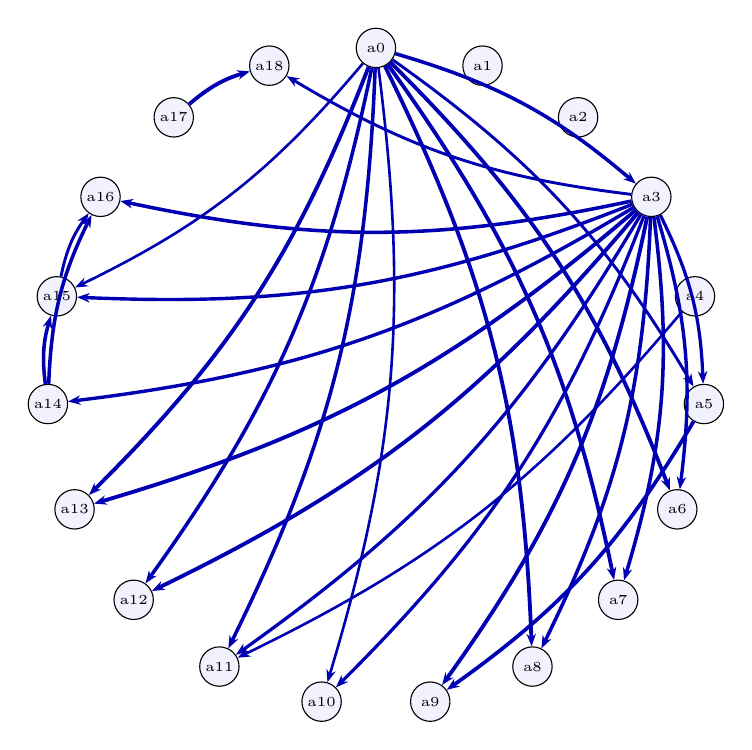
\begin{tikzpicture}[>={Stealth[length=1.6mm]}]
  \node[circle,draw,fill=blue!5,inner sep=1pt,minimum size=5mm,font=\tiny] (a0) at (90.0:4.18) {a0};
  \node[circle,draw,fill=blue!5,inner sep=1pt,minimum size=5mm,font=\tiny] (a1) at (71.1:4.18) {a1};
  \node[circle,draw,fill=blue!5,inner sep=1pt,minimum size=5mm,font=\tiny] (a2) at (52.1:4.18) {a2};
  \node[circle,draw,fill=blue!5,inner sep=1pt,minimum size=5mm,font=\tiny] (a3) at (33.2:4.18) {a3};
  \node[circle,draw,fill=blue!5,inner sep=1pt,minimum size=5mm,font=\tiny] (a4) at (14.2:4.18) {a4};
  \node[circle,draw,fill=blue!5,inner sep=1pt,minimum size=5mm,font=\tiny] (a5) at (-4.7:4.18) {a5};
  \node[circle,draw,fill=blue!5,inner sep=1pt,minimum size=5mm,font=\tiny] (a6) at (-23.7:4.18) {a6};
  \node[circle,draw,fill=blue!5,inner sep=1pt,minimum size=5mm,font=\tiny] (a7) at (-42.6:4.18) {a7};
  \node[circle,draw,fill=blue!5,inner sep=1pt,minimum size=5mm,font=\tiny] (a8) at (-61.6:4.18) {a8};
  \node[circle,draw,fill=blue!5,inner sep=1pt,minimum size=5mm,font=\tiny] (a9) at (-80.5:4.18) {a9};
  \node[circle,draw,fill=blue!5,inner sep=1pt,minimum size=5mm,font=\tiny] (a10) at (-99.5:4.18) {a10};
  \node[circle,draw,fill=blue!5,inner sep=1pt,minimum size=5mm,font=\tiny] (a11) at (-118.4:4.18) {a11};
  \node[circle,draw,fill=blue!5,inner sep=1pt,minimum size=5mm,font=\tiny] (a12) at (-137.4:4.18) {a12};
  \node[circle,draw,fill=blue!5,inner sep=1pt,minimum size=5mm,font=\tiny] (a13) at (-156.3:4.18) {a13};
  \node[circle,draw,fill=blue!5,inner sep=1pt,minimum size=5mm,font=\tiny] (a14) at (-175.3:4.18) {a14};
  \node[circle,draw,fill=blue!5,inner sep=1pt,minimum size=5mm,font=\tiny] (a15) at (-194.2:4.18) {a15};
  \node[circle,draw,fill=blue!5,inner sep=1pt,minimum size=5mm,font=\tiny] (a16) at (-213.2:4.18) {a16};
  \node[circle,draw,fill=blue!5,inner sep=1pt,minimum size=5mm,font=\tiny] (a17) at (-232.1:4.18) {a17};
  \node[circle,draw,fill=blue!5,inner sep=1pt,minimum size=5mm,font=\tiny] (a18) at (-251.1:4.18) {a18};
  \draw[-{Stealth[length=1.6mm]}, blue!70!black, line width=1.28pt] (a0) to[bend left=12] (a3);
  \draw[-{Stealth[length=1.6mm]}, blue!70!black, line width=1.17pt] (a3) to[bend left=12] (a5);
  \draw[-{Stealth[length=1.6mm]}, blue!70!black, line width=1.23pt] (a3) to[bend left=12] (a6);
  \draw[-{Stealth[length=1.6mm]}, blue!70!black, line width=1.28pt] (a3) to[bend left=12] (a7);
  \draw[-{Stealth[length=1.6mm]}, blue!70!black, line width=1.34pt] (a5) to[bend left=12] (a9);
  \draw[-{Stealth[length=1.6mm]}, blue!70!black, line width=1.28pt] (a14) to[bend left=12] (a15);
  \draw[-{Stealth[length=1.6mm]}, blue!70!black, line width=1.28pt] (a14) to[bend left=12] (a16);
  \draw[-{Stealth[length=1.6mm]}, blue!70!black, line width=1.05pt] (a15) to[bend left=12] (a16);
  \draw[-{Stealth[length=1.6mm]}, blue!70!black, line width=1.38pt] (a17) to[bend left=12] (a18);
  \draw[-{Stealth[length=1.6mm]}, blue!70!black, line width=1.17pt] (a3) to[bend left=12] (a10);
  \draw[-{Stealth[length=1.6mm]}, blue!70!black, line width=1.17pt] (a3) to[bend left=12] (a11);
  \draw[-{Stealth[length=1.6mm]}, blue!70!black, line width=1.39pt] (a3) to[bend left=12] (a12);
  \draw[-{Stealth[length=1.6mm]}, blue!70!black, line width=1.40pt] (a3) to[bend left=12] (a13);
  \draw[-{Stealth[length=1.6mm]}, blue!70!black, line width=1.23pt] (a3) to[bend left=12] (a15);
  \draw[-{Stealth[length=1.6mm]}, blue!70!black, line width=1.05pt] (a0) to[bend left=12] (a5);
  \draw[-{Stealth[length=1.6mm]}, blue!70!black, line width=1.38pt] (a0) to[bend left=12] (a6);
  \draw[-{Stealth[length=1.6mm]}, blue!70!black, line width=1.38pt] (a0) to[bend left=12] (a7);
  \draw[-{Stealth[length=1.6mm]}, blue!70!black, line width=1.38pt] (a0) to[bend left=12] (a8);
  \draw[-{Stealth[length=1.6mm]}, blue!70!black, line width=0.94pt] (a0) to[bend left=12] (a10);
  \draw[-{Stealth[length=1.6mm]}, blue!70!black, line width=1.28pt] (a0) to[bend left=12] (a11);
  \draw[-{Stealth[length=1.6mm]}, blue!70!black, line width=1.28pt] (a0) to[bend left=12] (a12);
  \draw[-{Stealth[length=1.6mm]}, blue!70!black, line width=1.40pt] (a0) to[bend left=12] (a13);
  \draw[-{Stealth[length=1.6mm]}, blue!70!black, line width=0.94pt] (a0) to[bend left=12] (a15);
  \draw[-{Stealth[length=1.6mm]}, blue!70!black, line width=1.28pt] (a3) to[bend left=12] (a8);
  \draw[-{Stealth[length=1.6mm]}, blue!70!black, line width=1.38pt] (a3) to[bend left=12] (a9);
  \draw[-{Stealth[length=1.6mm]}, blue!70!black, line width=1.23pt] (a3) to[bend left=12] (a14);
  \draw[-{Stealth[length=1.6mm]}, blue!70!black, line width=1.28pt] (a3) to[bend left=12] (a16);
  \draw[-{Stealth[length=1.6mm]}, blue!70!black, line width=1.05pt] (a3) to[bend left=12] (a18);
  \draw[-{Stealth[length=1.6mm]}, blue!70!black, line width=0.94pt] (a4) to[bend left=12] (a11);
\end{tikzpicture}
}
\\[2pt]{\footnotesize gate: 29 relations}
\end{minipage}
\caption{Relation graph for \texttt{e2-bio} (Biography (consistent)): gate.}
\label{fig:graph-example-2-biography}
\end{figure}

\begin{figure}[htbp]
\centering
\begin{minipage}[t]{0.48\linewidth}\centering
\resizebox{!}{6.2cm}{%
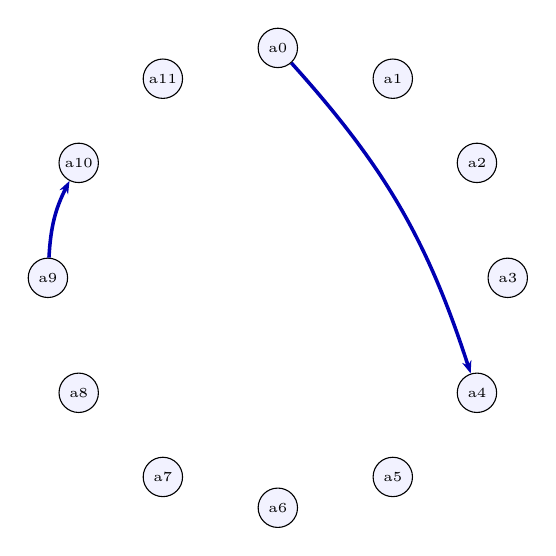
\begin{tikzpicture}[>={Stealth[length=1.6mm]}]
  \node[circle,draw,fill=blue!5,inner sep=1pt,minimum size=5mm,font=\tiny] (a0) at (90.0:2.92) {a0};
  \node[circle,draw,fill=blue!5,inner sep=1pt,minimum size=5mm,font=\tiny] (a1) at (60.0:2.92) {a1};
  \node[circle,draw,fill=blue!5,inner sep=1pt,minimum size=5mm,font=\tiny] (a2) at (30.0:2.92) {a2};
  \node[circle,draw,fill=blue!5,inner sep=1pt,minimum size=5mm,font=\tiny] (a3) at (0.0:2.92) {a3};
  \node[circle,draw,fill=blue!5,inner sep=1pt,minimum size=5mm,font=\tiny] (a4) at (-30.0:2.92) {a4};
  \node[circle,draw,fill=blue!5,inner sep=1pt,minimum size=5mm,font=\tiny] (a5) at (-60.0:2.92) {a5};
  \node[circle,draw,fill=blue!5,inner sep=1pt,minimum size=5mm,font=\tiny] (a6) at (-90.0:2.92) {a6};
  \node[circle,draw,fill=blue!5,inner sep=1pt,minimum size=5mm,font=\tiny] (a7) at (-120.0:2.92) {a7};
  \node[circle,draw,fill=blue!5,inner sep=1pt,minimum size=5mm,font=\tiny] (a8) at (-150.0:2.92) {a8};
  \node[circle,draw,fill=blue!5,inner sep=1pt,minimum size=5mm,font=\tiny] (a9) at (-180.0:2.92) {a9};
  \node[circle,draw,fill=blue!5,inner sep=1pt,minimum size=5mm,font=\tiny] (a10) at (-210.0:2.92) {a10};
  \node[circle,draw,fill=blue!5,inner sep=1pt,minimum size=5mm,font=\tiny] (a11) at (-240.0:2.92) {a11};
  \draw[-{Stealth[length=1.6mm]}, blue!70!black, line width=1.28pt] (a0) to[bend left=12] (a4);
  \draw[-{Stealth[length=1.6mm]}, blue!70!black, line width=1.28pt] (a9) to[bend left=12] (a10);
\end{tikzpicture}
}
\\[2pt]{\footnotesize gate: 2 relations}
\end{minipage}
\caption{Relation graph for \texttt{e2-con} (Biography (with planted contradictions)): gate.}
\label{fig:graph-example-2-biography-contradicted}
\end{figure}

\begin{figure}[htbp]
\centering
\begin{minipage}[t]{0.48\linewidth}\centering
\resizebox{!}{6.2cm}{%
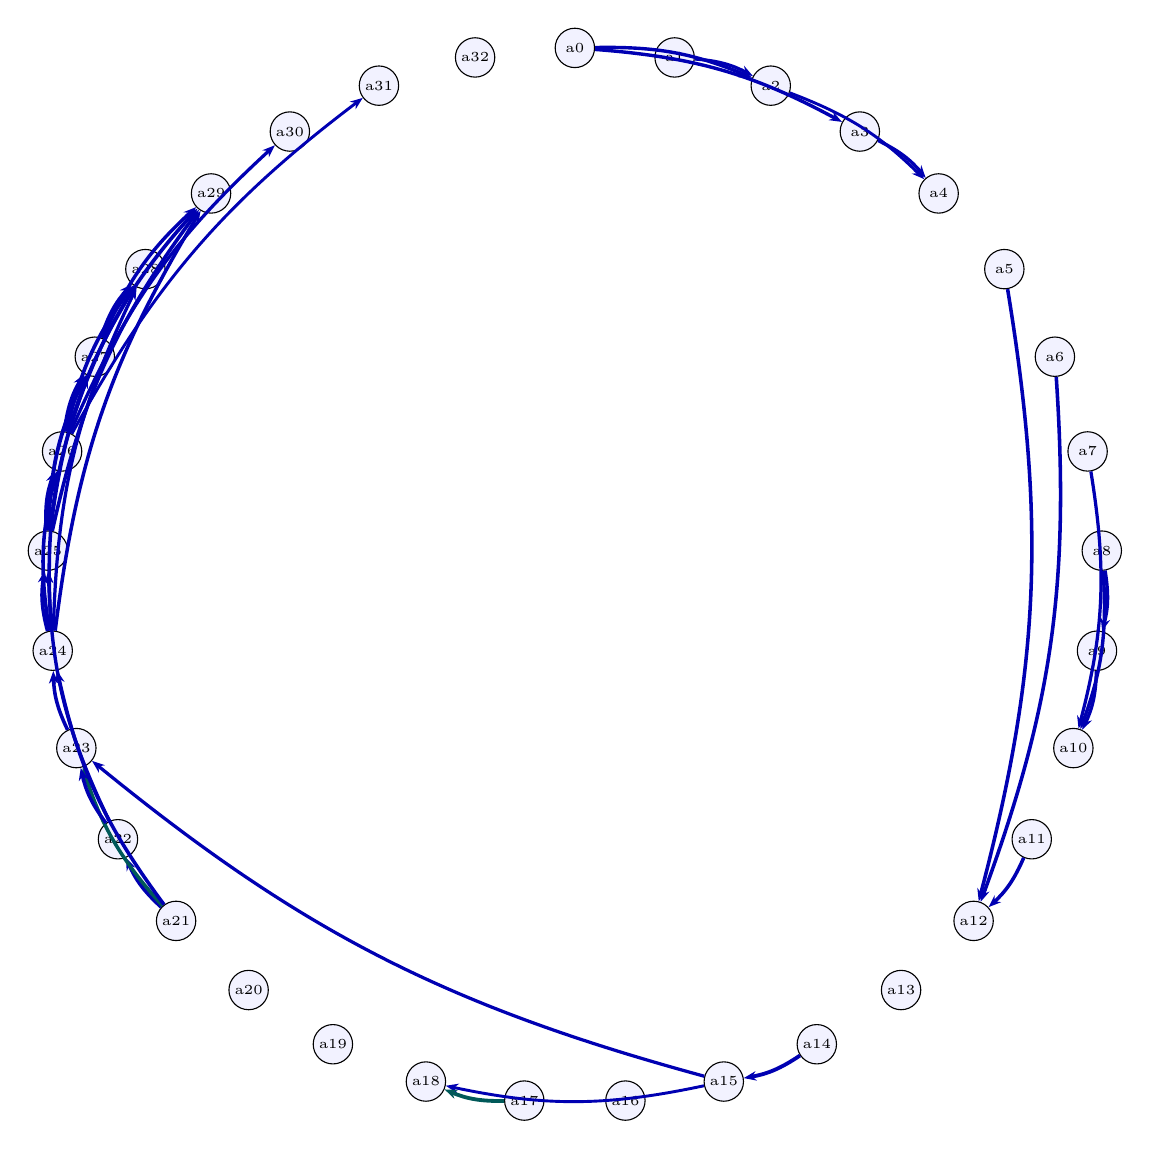
\begin{tikzpicture}[>={Stealth[length=1.6mm]}]
  \node[circle,draw,fill=blue!5,inner sep=1pt,minimum size=5mm,font=\tiny] (a0) at (90.0:6.70) {a0};
  \node[circle,draw,fill=blue!5,inner sep=1pt,minimum size=5mm,font=\tiny] (a1) at (79.1:6.70) {a1};
  \node[circle,draw,fill=blue!5,inner sep=1pt,minimum size=5mm,font=\tiny] (a2) at (68.2:6.70) {a2};
  \node[circle,draw,fill=blue!5,inner sep=1pt,minimum size=5mm,font=\tiny] (a3) at (57.3:6.70) {a3};
  \node[circle,draw,fill=blue!5,inner sep=1pt,minimum size=5mm,font=\tiny] (a4) at (46.4:6.70) {a4};
  \node[circle,draw,fill=blue!5,inner sep=1pt,minimum size=5mm,font=\tiny] (a5) at (35.5:6.70) {a5};
  \node[circle,draw,fill=blue!5,inner sep=1pt,minimum size=5mm,font=\tiny] (a6) at (24.5:6.70) {a6};
  \node[circle,draw,fill=blue!5,inner sep=1pt,minimum size=5mm,font=\tiny] (a7) at (13.6:6.70) {a7};
  \node[circle,draw,fill=blue!5,inner sep=1pt,minimum size=5mm,font=\tiny] (a8) at (2.7:6.70) {a8};
  \node[circle,draw,fill=blue!5,inner sep=1pt,minimum size=5mm,font=\tiny] (a9) at (-8.2:6.70) {a9};
  \node[circle,draw,fill=blue!5,inner sep=1pt,minimum size=5mm,font=\tiny] (a10) at (-19.1:6.70) {a10};
  \node[circle,draw,fill=blue!5,inner sep=1pt,minimum size=5mm,font=\tiny] (a11) at (-30.0:6.70) {a11};
  \node[circle,draw,fill=blue!5,inner sep=1pt,minimum size=5mm,font=\tiny] (a12) at (-40.9:6.70) {a12};
  \node[circle,draw,fill=blue!5,inner sep=1pt,minimum size=5mm,font=\tiny] (a13) at (-51.8:6.70) {a13};
  \node[circle,draw,fill=blue!5,inner sep=1pt,minimum size=5mm,font=\tiny] (a14) at (-62.7:6.70) {a14};
  \node[circle,draw,fill=blue!5,inner sep=1pt,minimum size=5mm,font=\tiny] (a15) at (-73.6:6.70) {a15};
  \node[circle,draw,fill=blue!5,inner sep=1pt,minimum size=5mm,font=\tiny] (a16) at (-84.5:6.70) {a16};
  \node[circle,draw,fill=blue!5,inner sep=1pt,minimum size=5mm,font=\tiny] (a17) at (-95.5:6.70) {a17};
  \node[circle,draw,fill=blue!5,inner sep=1pt,minimum size=5mm,font=\tiny] (a18) at (-106.4:6.70) {a18};
  \node[circle,draw,fill=blue!5,inner sep=1pt,minimum size=5mm,font=\tiny] (a19) at (-117.3:6.70) {a19};
  \node[circle,draw,fill=blue!5,inner sep=1pt,minimum size=5mm,font=\tiny] (a20) at (-128.2:6.70) {a20};
  \node[circle,draw,fill=blue!5,inner sep=1pt,minimum size=5mm,font=\tiny] (a21) at (-139.1:6.70) {a21};
  \node[circle,draw,fill=blue!5,inner sep=1pt,minimum size=5mm,font=\tiny] (a22) at (-150.0:6.70) {a22};
  \node[circle,draw,fill=blue!5,inner sep=1pt,minimum size=5mm,font=\tiny] (a23) at (-160.9:6.70) {a23};
  \node[circle,draw,fill=blue!5,inner sep=1pt,minimum size=5mm,font=\tiny] (a24) at (-171.8:6.70) {a24};
  \node[circle,draw,fill=blue!5,inner sep=1pt,minimum size=5mm,font=\tiny] (a25) at (-182.7:6.70) {a25};
  \node[circle,draw,fill=blue!5,inner sep=1pt,minimum size=5mm,font=\tiny] (a26) at (-193.6:6.70) {a26};
  \node[circle,draw,fill=blue!5,inner sep=1pt,minimum size=5mm,font=\tiny] (a27) at (-204.5:6.70) {a27};
  \node[circle,draw,fill=blue!5,inner sep=1pt,minimum size=5mm,font=\tiny] (a28) at (-215.5:6.70) {a28};
  \node[circle,draw,fill=blue!5,inner sep=1pt,minimum size=5mm,font=\tiny] (a29) at (-226.4:6.70) {a29};
  \node[circle,draw,fill=blue!5,inner sep=1pt,minimum size=5mm,font=\tiny] (a30) at (-237.3:6.70) {a30};
  \node[circle,draw,fill=blue!5,inner sep=1pt,minimum size=5mm,font=\tiny] (a31) at (-248.2:6.70) {a31};
  \node[circle,draw,fill=blue!5,inner sep=1pt,minimum size=5mm,font=\tiny] (a32) at (-259.1:6.70) {a32};
  \draw[-{Stealth[length=1.6mm]}, blue!70!black, line width=1.23pt] (a0) to[bend left=12] (a2);
  \draw[-{Stealth[length=1.6mm]}, blue!70!black, line width=1.23pt] (a0) to[bend left=12] (a3);
  \draw[-{Stealth[length=1.6mm]}, blue!70!black, line width=1.17pt] (a1) to[bend left=12] (a2);
  \draw[-{Stealth[length=1.6mm]}, blue!70!black, line width=1.05pt] (a2) to[bend left=12] (a4);
  \draw[-{Stealth[length=1.6mm]}, blue!70!black, line width=1.23pt] (a3) to[bend left=12] (a4);
  \draw[-{Stealth[length=1.6mm]}, blue!70!black, line width=1.17pt] (a7) to[bend left=12] (a10);
  \draw[-{Stealth[length=1.6mm]}, blue!70!black, line width=1.23pt] (a8) to[bend left=12] (a9);
  \draw[-{Stealth[length=1.6mm]}, blue!70!black, line width=1.23pt] (a8) to[bend left=12] (a10);
  \draw[-{Stealth[length=1.6mm]}, blue!70!black, line width=1.23pt] (a9) to[bend left=12] (a10);
  \draw[-{Stealth[length=1.6mm]}, blue!70!black, line width=1.28pt] (a11) to[bend left=12] (a12);
  \draw[-{Stealth[length=1.6mm]}, blue!70!black, line width=1.38pt] (a14) to[bend left=12] (a15);
  \draw[-{Stealth[length=1.6mm]}, blue!70!black, line width=1.05pt] (a15) to[bend left=12] (a18);
  \draw[-{Stealth[length=1.6mm]}, teal!70!black, line width=1.38pt] (a17) to[bend left=12] (a18);
  \draw[-{Stealth[length=1.6mm]}, blue!70!black, line width=1.28pt] (a21) to[bend left=12] (a22);
  \draw[-{Stealth[length=1.6mm]}, teal!70!black, line width=1.28pt] (a21) to[bend left=12] (a23);
  \draw[-{Stealth[length=1.6mm]}, blue!70!black, line width=1.28pt] (a21) to[bend left=12] (a24);
  \draw[-{Stealth[length=1.6mm]}, blue!70!black, line width=1.28pt] (a22) to[bend left=12] (a23);
  \draw[-{Stealth[length=1.6mm]}, blue!70!black, line width=1.23pt] (a22) to[bend left=12] (a25);
  \draw[-{Stealth[length=1.6mm]}, blue!70!black, line width=1.28pt] (a23) to[bend left=12] (a24);
  \draw[-{Stealth[length=1.6mm]}, blue!70!black, line width=1.28pt] (a24) to[bend left=12] (a25);
  \draw[-{Stealth[length=1.6mm]}, blue!70!black, line width=1.28pt] (a24) to[bend left=12] (a26);
  \draw[-{Stealth[length=1.6mm]}, blue!70!black, line width=1.28pt] (a24) to[bend left=12] (a27);
  \draw[-{Stealth[length=1.6mm]}, blue!70!black, line width=1.17pt] (a24) to[bend left=12] (a28);
  \draw[-{Stealth[length=1.6mm]}, blue!70!black, line width=1.38pt] (a25) to[bend left=12] (a26);
  \draw[-{Stealth[length=1.6mm]}, blue!70!black, line width=1.38pt] (a25) to[bend left=12] (a27);
  \draw[-{Stealth[length=1.6mm]}, blue!70!black, line width=1.28pt] (a25) to[bend left=12] (a28);
  \draw[-{Stealth[length=1.6mm]}, blue!70!black, line width=1.28pt] (a25) to[bend left=12] (a29);
  \draw[-{Stealth[length=1.6mm]}, blue!70!black, line width=1.38pt] (a26) to[bend left=12] (a27);
  \draw[-{Stealth[length=1.6mm]}, blue!70!black, line width=1.31pt] (a26) to[bend left=12] (a28);
  \draw[-{Stealth[length=1.6mm]}, blue!70!black, line width=1.31pt] (a26) to[bend left=12] (a29);
  \draw[-{Stealth[length=1.6mm]}, blue!70!black, line width=1.17pt] (a26) to[bend left=12] (a30);
  \draw[-{Stealth[length=1.6mm]}, blue!70!black, line width=1.23pt] (a27) to[bend left=12] (a28);
  \draw[-{Stealth[length=1.6mm]}, blue!70!black, line width=1.23pt] (a27) to[bend left=12] (a29);
  \draw[-{Stealth[length=1.6mm]}, blue!70!black, line width=1.28pt] (a5) to[bend left=12] (a12);
  \draw[-{Stealth[length=1.6mm]}, blue!70!black, line width=1.28pt] (a6) to[bend left=12] (a12);
  \draw[-{Stealth[length=1.6mm]}, blue!70!black, line width=1.17pt] (a15) to[bend left=12] (a23);
  \draw[-{Stealth[length=1.6mm]}, blue!70!black, line width=1.26pt] (a24) to[bend left=12] (a29);
  \draw[-{Stealth[length=1.6mm]}, blue!70!black, line width=1.05pt] (a26) to[bend left=12] (a31);
\end{tikzpicture}
}
\\[2pt]{\footnotesize gate: 38 relations}
\end{minipage}
\caption{Relation graph for \texttt{e3-nar} (Narrative passage (Elinor)): gate.}
\label{fig:graph-example-3-narrative}
\end{figure}

\begin{figure}[htbp]
\centering
\begin{minipage}[t]{0.48\linewidth}\centering
\resizebox{!}{6.2cm}{%
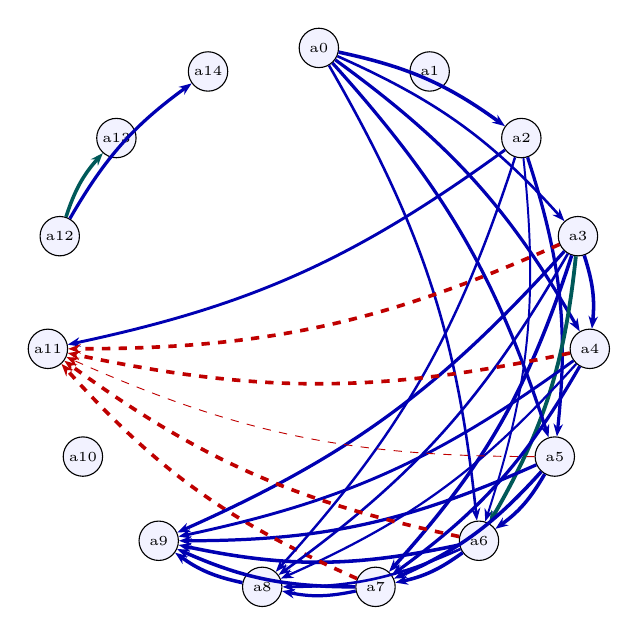
\begin{tikzpicture}[>={Stealth[length=1.6mm]}]
  \node[circle,draw,fill=blue!5,inner sep=1pt,minimum size=5mm,font=\tiny] (a0) at (90.0:3.46) {a0};
  \node[circle,draw,fill=blue!5,inner sep=1pt,minimum size=5mm,font=\tiny] (a1) at (66.0:3.46) {a1};
  \node[circle,draw,fill=blue!5,inner sep=1pt,minimum size=5mm,font=\tiny] (a2) at (42.0:3.46) {a2};
  \node[circle,draw,fill=blue!5,inner sep=1pt,minimum size=5mm,font=\tiny] (a3) at (18.0:3.46) {a3};
  \node[circle,draw,fill=blue!5,inner sep=1pt,minimum size=5mm,font=\tiny] (a4) at (-6.0:3.46) {a4};
  \node[circle,draw,fill=blue!5,inner sep=1pt,minimum size=5mm,font=\tiny] (a5) at (-30.0:3.46) {a5};
  \node[circle,draw,fill=blue!5,inner sep=1pt,minimum size=5mm,font=\tiny] (a6) at (-54.0:3.46) {a6};
  \node[circle,draw,fill=blue!5,inner sep=1pt,minimum size=5mm,font=\tiny] (a7) at (-78.0:3.46) {a7};
  \node[circle,draw,fill=blue!5,inner sep=1pt,minimum size=5mm,font=\tiny] (a8) at (-102.0:3.46) {a8};
  \node[circle,draw,fill=blue!5,inner sep=1pt,minimum size=5mm,font=\tiny] (a9) at (-126.0:3.46) {a9};
  \node[circle,draw,fill=blue!5,inner sep=1pt,minimum size=5mm,font=\tiny] (a10) at (-150.0:3.46) {a10};
  \node[circle,draw,fill=blue!5,inner sep=1pt,minimum size=5mm,font=\tiny] (a11) at (-174.0:3.46) {a11};
  \node[circle,draw,fill=blue!5,inner sep=1pt,minimum size=5mm,font=\tiny] (a12) at (-198.0:3.46) {a12};
  \node[circle,draw,fill=blue!5,inner sep=1pt,minimum size=5mm,font=\tiny] (a13) at (-222.0:3.46) {a13};
  \node[circle,draw,fill=blue!5,inner sep=1pt,minimum size=5mm,font=\tiny] (a14) at (-246.0:3.46) {a14};
  \draw[-{Stealth[length=1.6mm]}, blue!70!black, line width=1.28pt] (a0) to[bend left=12] (a2);
  \draw[-{Stealth[length=1.6mm]}, blue!70!black, line width=0.94pt] (a0) to[bend left=12] (a3);
  \draw[-{Stealth[length=1.6mm]}, blue!70!black, line width=1.17pt] (a0) to[bend left=12] (a4);
  \draw[-{Stealth[length=1.6mm]}, blue!70!black, line width=1.17pt] (a2) to[bend left=12] (a5);
  \draw[-{Stealth[length=1.6mm]}, blue!70!black, line width=0.71pt] (a2) to[bend left=12] (a6);
  \draw[-{Stealth[length=1.6mm]}, blue!70!black, line width=1.28pt] (a3) to[bend left=12] (a4);
  \draw[-{Stealth[length=1.6mm]}, teal!70!black, line width=1.38pt] (a3) to[bend left=12] (a6);
  \draw[-{Stealth[length=1.6mm]}, blue!70!black, line width=1.28pt] (a3) to[bend left=12] (a7);
  \draw[-{Stealth[length=1.6mm]}, blue!70!black, line width=1.17pt] (a4) to[bend left=12] (a7);
  \draw[-{Stealth[length=1.6mm]}, blue!70!black, line width=0.82pt] (a4) to[bend left=12] (a8);
  \draw[-{Stealth[length=1.6mm]}, blue!70!black, line width=1.28pt] (a5) to[bend left=12] (a6);
  \draw[-{Stealth[length=1.6mm]}, blue!70!black, line width=1.28pt] (a5) to[bend left=12] (a7);
  \draw[-{Stealth[length=1.6mm]}, blue!70!black, line width=1.17pt] (a5) to[bend left=12] (a9);
  \draw[-{Stealth[length=1.6mm]}, blue!70!black, line width=1.28pt] (a6) to[bend left=12] (a7);
  \draw[-{Stealth[length=1.6mm]}, blue!70!black, line width=0.94pt] (a6) to[bend left=12] (a8);
  \draw[-{Stealth[length=1.6mm]}, blue!70!black, line width=1.28pt] (a6) to[bend left=12] (a9);
  \draw[-{Stealth[length=1.6mm]}, blue!70!black, line width=1.17pt] (a7) to[bend left=12] (a8);
  \draw[-{Stealth[length=1.6mm]}, blue!70!black, line width=1.28pt] (a7) to[bend left=12] (a9);
  \draw[-{Stealth[length=1.6mm]}, red!75!black, dashed, line width=1.32pt] (a7) to[bend left=12] (a11);
  \draw[-{Stealth[length=1.6mm]}, blue!70!black, line width=1.28pt] (a8) to[bend left=12] (a9);
  \draw[-{Stealth[length=1.6mm]}, teal!70!black, line width=1.28pt] (a12) to[bend left=12] (a13);
  \draw[-{Stealth[length=1.6mm]}, blue!70!black, line width=1.17pt] (a12) to[bend left=12] (a14);
  \draw[-{Stealth[length=1.6mm]}, blue!70!black, line width=0.94pt] (a0) to[bend left=12] (a6);
  \draw[-{Stealth[length=1.6mm]}, blue!70!black, line width=1.05pt] (a2) to[bend left=12] (a11);
  \draw[-{Stealth[length=1.6mm]}, red!75!black, dashed, line width=1.32pt] (a3) to[bend left=12] (a11);
  \draw[-{Stealth[length=1.6mm]}, blue!70!black, line width=1.17pt] (a0) to[bend left=12] (a5);
  \draw[-{Stealth[length=1.6mm]}, blue!70!black, line width=0.88pt] (a2) to[bend left=12] (a8);
  \draw[-{Stealth[length=1.6mm]}, blue!70!black, line width=0.94pt] (a3) to[bend left=12] (a8);
  \draw[-{Stealth[length=1.6mm]}, blue!70!black, line width=1.17pt] (a3) to[bend left=12] (a9);
  \draw[-{Stealth[length=1.6mm]}, blue!70!black, line width=1.05pt] (a4) to[bend left=12] (a9);
  \draw[-{Stealth[length=1.6mm]}, red!75!black, dashed, line width=1.32pt] (a4) to[bend left=12] (a11);
  \draw[-{Stealth[length=1.6mm]}, red!75!black, dashed, line width=0.33pt] (a5) to[bend left=12] (a11);
  \draw[-{Stealth[length=1.6mm]}, red!75!black, dashed, line width=1.32pt] (a6) to[bend left=12] (a11);
\end{tikzpicture}
}
\\[2pt]{\footnotesize gate: 33 relations}
\end{minipage}
\caption{Relation graph for \texttt{e4-sum} (Synthesized summary S (reliable + unreliable sources)): gate.}
\label{fig:graph-example-4-summary}
\end{figure}

\begin{figure}[htbp]
\centering
\begin{minipage}[t]{0.48\linewidth}\centering
\resizebox{!}{6.2cm}{%
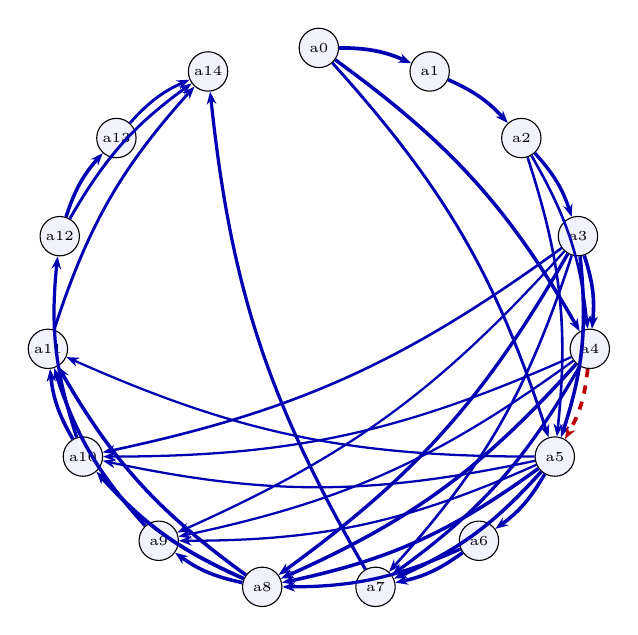
\begin{tikzpicture}[>={Stealth[length=1.6mm]}]
  \node[circle,draw,fill=blue!5,inner sep=1pt,minimum size=5mm,font=\tiny] (a0) at (90.0:3.46) {a0};
  \node[circle,draw,fill=blue!5,inner sep=1pt,minimum size=5mm,font=\tiny] (a1) at (66.0:3.46) {a1};
  \node[circle,draw,fill=blue!5,inner sep=1pt,minimum size=5mm,font=\tiny] (a2) at (42.0:3.46) {a2};
  \node[circle,draw,fill=blue!5,inner sep=1pt,minimum size=5mm,font=\tiny] (a3) at (18.0:3.46) {a3};
  \node[circle,draw,fill=blue!5,inner sep=1pt,minimum size=5mm,font=\tiny] (a4) at (-6.0:3.46) {a4};
  \node[circle,draw,fill=blue!5,inner sep=1pt,minimum size=5mm,font=\tiny] (a5) at (-30.0:3.46) {a5};
  \node[circle,draw,fill=blue!5,inner sep=1pt,minimum size=5mm,font=\tiny] (a6) at (-54.0:3.46) {a6};
  \node[circle,draw,fill=blue!5,inner sep=1pt,minimum size=5mm,font=\tiny] (a7) at (-78.0:3.46) {a7};
  \node[circle,draw,fill=blue!5,inner sep=1pt,minimum size=5mm,font=\tiny] (a8) at (-102.0:3.46) {a8};
  \node[circle,draw,fill=blue!5,inner sep=1pt,minimum size=5mm,font=\tiny] (a9) at (-126.0:3.46) {a9};
  \node[circle,draw,fill=blue!5,inner sep=1pt,minimum size=5mm,font=\tiny] (a10) at (-150.0:3.46) {a10};
  \node[circle,draw,fill=blue!5,inner sep=1pt,minimum size=5mm,font=\tiny] (a11) at (-174.0:3.46) {a11};
  \node[circle,draw,fill=blue!5,inner sep=1pt,minimum size=5mm,font=\tiny] (a12) at (-198.0:3.46) {a12};
  \node[circle,draw,fill=blue!5,inner sep=1pt,minimum size=5mm,font=\tiny] (a13) at (-222.0:3.46) {a13};
  \node[circle,draw,fill=blue!5,inner sep=1pt,minimum size=5mm,font=\tiny] (a14) at (-246.0:3.46) {a14};
  \draw[-{Stealth[length=1.6mm]}, blue!70!black, line width=1.34pt] (a0) to[bend left=12] (a1);
  \draw[-{Stealth[length=1.6mm]}, blue!70!black, line width=1.28pt] (a0) to[bend left=12] (a4);
  \draw[-{Stealth[length=1.6mm]}, blue!70!black, line width=1.28pt] (a1) to[bend left=12] (a2);
  \draw[-{Stealth[length=1.6mm]}, blue!70!black, line width=1.23pt] (a2) to[bend left=12] (a3);
  \draw[-{Stealth[length=1.6mm]}, blue!70!black, line width=0.94pt] (a2) to[bend left=12] (a4);
  \draw[-{Stealth[length=1.6mm]}, blue!70!black, line width=0.94pt] (a2) to[bend left=12] (a5);
  \draw[-{Stealth[length=1.6mm]}, blue!70!black, line width=1.31pt] (a3) to[bend left=12] (a4);
  \draw[-{Stealth[length=1.6mm]}, blue!70!black, line width=1.28pt] (a3) to[bend left=12] (a5);
  \draw[-{Stealth[length=1.6mm]}, blue!70!black, line width=0.94pt] (a3) to[bend left=12] (a7);
  \draw[-{Stealth[length=1.6mm]}, red!75!black, dashed, line width=1.34pt] (a4) to[bend left=12] (a5);
  \draw[-{Stealth[length=1.6mm]}, blue!70!black, line width=1.17pt] (a4) to[bend left=12] (a7);
  \draw[-{Stealth[length=1.6mm]}, blue!70!black, line width=1.28pt] (a4) to[bend left=12] (a8);
  \draw[-{Stealth[length=1.6mm]}, blue!70!black, line width=1.28pt] (a5) to[bend left=12] (a6);
  \draw[-{Stealth[length=1.6mm]}, blue!70!black, line width=1.28pt] (a5) to[bend left=12] (a7);
  \draw[-{Stealth[length=1.6mm]}, blue!70!black, line width=1.28pt] (a5) to[bend left=12] (a8);
  \draw[-{Stealth[length=1.6mm]}, blue!70!black, line width=0.82pt] (a5) to[bend left=12] (a9);
  \draw[-{Stealth[length=1.6mm]}, blue!70!black, line width=1.28pt] (a6) to[bend left=12] (a7);
  \draw[-{Stealth[length=1.6mm]}, blue!70!black, line width=1.17pt] (a6) to[bend left=12] (a8);
  \draw[-{Stealth[length=1.6mm]}, blue!70!black, line width=1.28pt] (a8) to[bend left=12] (a9);
  \draw[-{Stealth[length=1.6mm]}, blue!70!black, line width=1.38pt] (a8) to[bend left=12] (a10);
  \draw[-{Stealth[length=1.6mm]}, blue!70!black, line width=1.28pt] (a8) to[bend left=12] (a11);
  \draw[-{Stealth[length=1.6mm]}, blue!70!black, line width=1.28pt] (a9) to[bend left=12] (a11);
  \draw[-{Stealth[length=1.6mm]}, blue!70!black, line width=1.28pt] (a10) to[bend left=12] (a11);
  \draw[-{Stealth[length=1.6mm]}, blue!70!black, line width=1.17pt] (a10) to[bend left=12] (a12);
  \draw[-{Stealth[length=1.6mm]}, blue!70!black, line width=1.05pt] (a11) to[bend left=12] (a14);
  \draw[-{Stealth[length=1.6mm]}, blue!70!black, line width=1.28pt] (a12) to[bend left=12] (a13);
  \draw[-{Stealth[length=1.6mm]}, blue!70!black, line width=1.05pt] (a12) to[bend left=12] (a14);
  \draw[-{Stealth[length=1.6mm]}, blue!70!black, line width=1.05pt] (a13) to[bend left=12] (a14);
  \draw[-{Stealth[length=1.6mm]}, blue!70!black, line width=1.05pt] (a0) to[bend left=12] (a5);
  \draw[-{Stealth[length=1.6mm]}, blue!70!black, line width=1.23pt] (a3) to[bend left=12] (a8);
  \draw[-{Stealth[length=1.6mm]}, blue!70!black, line width=0.82pt] (a3) to[bend left=12] (a9);
  \draw[-{Stealth[length=1.6mm]}, blue!70!black, line width=0.94pt] (a3) to[bend left=12] (a10);
  \draw[-{Stealth[length=1.6mm]}, blue!70!black, line width=0.82pt] (a4) to[bend left=12] (a9);
  \draw[-{Stealth[length=1.6mm]}, blue!70!black, line width=0.82pt] (a4) to[bend left=12] (a10);
  \draw[-{Stealth[length=1.6mm]}, blue!70!black, line width=0.82pt] (a5) to[bend left=12] (a10);
  \draw[-{Stealth[length=1.6mm]}, blue!70!black, line width=0.82pt] (a5) to[bend left=12] (a11);
  \draw[-{Stealth[length=1.6mm]}, blue!70!black, line width=1.17pt] (a7) to[bend left=12] (a14);
\end{tikzpicture}
}
\\[2pt]{\footnotesize gate: 37 relations}
\end{minipage}
\caption{Relation graph for \texttt{e5-K} (R v Renda summary K (faithful natural ordering)): gate.}
\label{fig:graph-example-5-renda-K}
\end{figure}

\begin{figure}[htbp]
\centering
\begin{minipage}[t]{0.48\linewidth}\centering
\resizebox{!}{6.2cm}{%
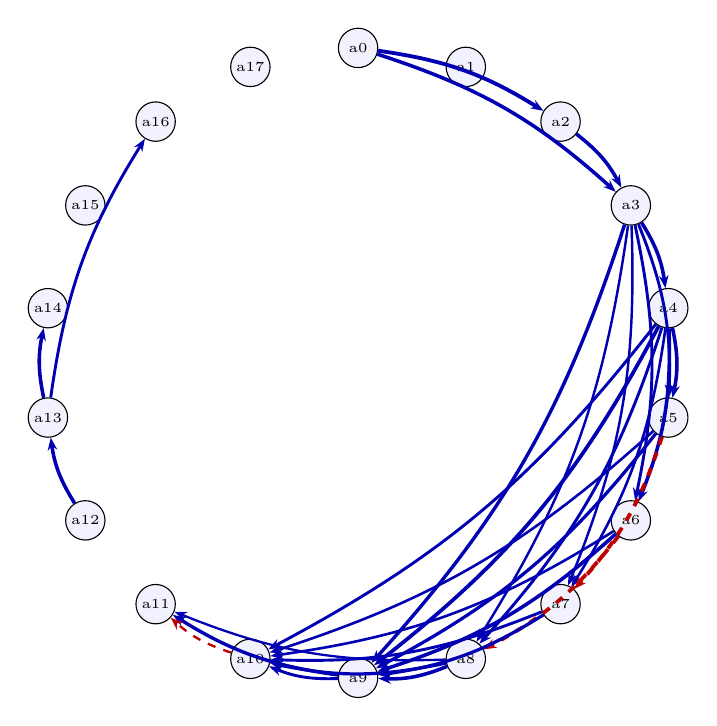
\begin{tikzpicture}[>={Stealth[length=1.6mm]}]
  \node[circle,draw,fill=blue!5,inner sep=1pt,minimum size=5mm,font=\tiny] (a0) at (90.0:4.00) {a0};
  \node[circle,draw,fill=blue!5,inner sep=1pt,minimum size=5mm,font=\tiny] (a1) at (70.0:4.00) {a1};
  \node[circle,draw,fill=blue!5,inner sep=1pt,minimum size=5mm,font=\tiny] (a2) at (50.0:4.00) {a2};
  \node[circle,draw,fill=blue!5,inner sep=1pt,minimum size=5mm,font=\tiny] (a3) at (30.0:4.00) {a3};
  \node[circle,draw,fill=blue!5,inner sep=1pt,minimum size=5mm,font=\tiny] (a4) at (10.0:4.00) {a4};
  \node[circle,draw,fill=blue!5,inner sep=1pt,minimum size=5mm,font=\tiny] (a5) at (-10.0:4.00) {a5};
  \node[circle,draw,fill=blue!5,inner sep=1pt,minimum size=5mm,font=\tiny] (a6) at (-30.0:4.00) {a6};
  \node[circle,draw,fill=blue!5,inner sep=1pt,minimum size=5mm,font=\tiny] (a7) at (-50.0:4.00) {a7};
  \node[circle,draw,fill=blue!5,inner sep=1pt,minimum size=5mm,font=\tiny] (a8) at (-70.0:4.00) {a8};
  \node[circle,draw,fill=blue!5,inner sep=1pt,minimum size=5mm,font=\tiny] (a9) at (-90.0:4.00) {a9};
  \node[circle,draw,fill=blue!5,inner sep=1pt,minimum size=5mm,font=\tiny] (a10) at (-110.0:4.00) {a10};
  \node[circle,draw,fill=blue!5,inner sep=1pt,minimum size=5mm,font=\tiny] (a11) at (-130.0:4.00) {a11};
  \node[circle,draw,fill=blue!5,inner sep=1pt,minimum size=5mm,font=\tiny] (a12) at (-150.0:4.00) {a12};
  \node[circle,draw,fill=blue!5,inner sep=1pt,minimum size=5mm,font=\tiny] (a13) at (-170.0:4.00) {a13};
  \node[circle,draw,fill=blue!5,inner sep=1pt,minimum size=5mm,font=\tiny] (a14) at (-190.0:4.00) {a14};
  \node[circle,draw,fill=blue!5,inner sep=1pt,minimum size=5mm,font=\tiny] (a15) at (-210.0:4.00) {a15};
  \node[circle,draw,fill=blue!5,inner sep=1pt,minimum size=5mm,font=\tiny] (a16) at (-230.0:4.00) {a16};
  \node[circle,draw,fill=blue!5,inner sep=1pt,minimum size=5mm,font=\tiny] (a17) at (-250.0:4.00) {a17};
  \draw[-{Stealth[length=1.6mm]}, blue!70!black, line width=1.38pt] (a0) to[bend left=12] (a2);
  \draw[-{Stealth[length=1.6mm]}, blue!70!black, line width=1.28pt] (a0) to[bend left=12] (a3);
  \draw[-{Stealth[length=1.6mm]}, blue!70!black, line width=1.28pt] (a2) to[bend left=12] (a3);
  \draw[-{Stealth[length=1.6mm]}, blue!70!black, line width=1.28pt] (a3) to[bend left=12] (a4);
  \draw[-{Stealth[length=1.6mm]}, blue!70!black, line width=1.05pt] (a3) to[bend left=12] (a5);
  \draw[-{Stealth[length=1.6mm]}, blue!70!black, line width=1.05pt] (a3) to[bend left=12] (a6);
  \draw[-{Stealth[length=1.6mm]}, blue!70!black, line width=0.88pt] (a3) to[bend left=12] (a7);
  \draw[-{Stealth[length=1.6mm]}, blue!70!black, line width=1.28pt] (a4) to[bend left=12] (a5);
  \draw[-{Stealth[length=1.6mm]}, blue!70!black, line width=1.28pt] (a4) to[bend left=12] (a6);
  \draw[-{Stealth[length=1.6mm]}, blue!70!black, line width=0.94pt] (a4) to[bend left=12] (a7);
  \draw[-{Stealth[length=1.6mm]}, blue!70!black, line width=1.05pt] (a4) to[bend left=12] (a8);
  \draw[-{Stealth[length=1.6mm]}, red!75!black, dashed, line width=1.38pt] (a5) to[bend left=12] (a7);
  \draw[-{Stealth[length=1.6mm]}, blue!70!black, line width=1.17pt] (a5) to[bend left=12] (a9);
  \draw[-{Stealth[length=1.6mm]}, red!75!black, dashed, line width=1.34pt] (a6) to[bend left=12] (a8);
  \draw[-{Stealth[length=1.6mm]}, blue!70!black, line width=1.28pt] (a6) to[bend left=12] (a9);
  \draw[-{Stealth[length=1.6mm]}, blue!70!black, line width=0.94pt] (a6) to[bend left=12] (a10);
  \draw[-{Stealth[length=1.6mm]}, blue!70!black, line width=1.17pt] (a7) to[bend left=12] (a9);
  \draw[-{Stealth[length=1.6mm]}, blue!70!black, line width=1.05pt] (a7) to[bend left=12] (a10);
  \draw[-{Stealth[length=1.6mm]}, blue!70!black, line width=1.28pt] (a8) to[bend left=12] (a9);
  \draw[-{Stealth[length=1.6mm]}, blue!70!black, line width=1.17pt] (a8) to[bend left=12] (a10);
  \draw[-{Stealth[length=1.6mm]}, blue!70!black, line width=0.82pt] (a8) to[bend left=12] (a11);
  \draw[-{Stealth[length=1.6mm]}, blue!70!black, line width=1.05pt] (a9) to[bend left=12] (a10);
  \draw[-{Stealth[length=1.6mm]}, blue!70!black, line width=1.23pt] (a9) to[bend left=12] (a11);
  \draw[-{Stealth[length=1.6mm]}, red!75!black, dashed, line width=0.83pt] (a10) to[bend left=12] (a11);
  \draw[-{Stealth[length=1.6mm]}, blue!70!black, line width=1.28pt] (a12) to[bend left=12] (a13);
  \draw[-{Stealth[length=1.6mm]}, blue!70!black, line width=1.28pt] (a13) to[bend left=12] (a14);
  \draw[-{Stealth[length=1.6mm]}, blue!70!black, line width=1.05pt] (a13) to[bend left=12] (a16);
  \draw[-{Stealth[length=1.6mm]}, blue!70!black, line width=0.88pt] (a3) to[bend left=12] (a8);
  \draw[-{Stealth[length=1.6mm]}, blue!70!black, line width=1.23pt] (a3) to[bend left=12] (a9);
  \draw[-{Stealth[length=1.6mm]}, blue!70!black, line width=1.34pt] (a4) to[bend left=12] (a9);
  \draw[-{Stealth[length=1.6mm]}, blue!70!black, line width=1.05pt] (a4) to[bend left=12] (a10);
  \draw[-{Stealth[length=1.6mm]}, blue!70!black, line width=0.94pt] (a5) to[bend left=12] (a10);
\end{tikzpicture}
}
\\[2pt]{\footnotesize gate: 32 relations}
\end{minipage}
\caption{Relation graph for \texttt{e5-S} (R v Renda summary S (self-serving-first ordering)): gate.}
\label{fig:graph-example-5-renda-S}
\end{figure}

\begin{figure}[htbp]
\centering
\begin{minipage}[t]{0.48\linewidth}\centering
\resizebox{!}{6.2cm}{%
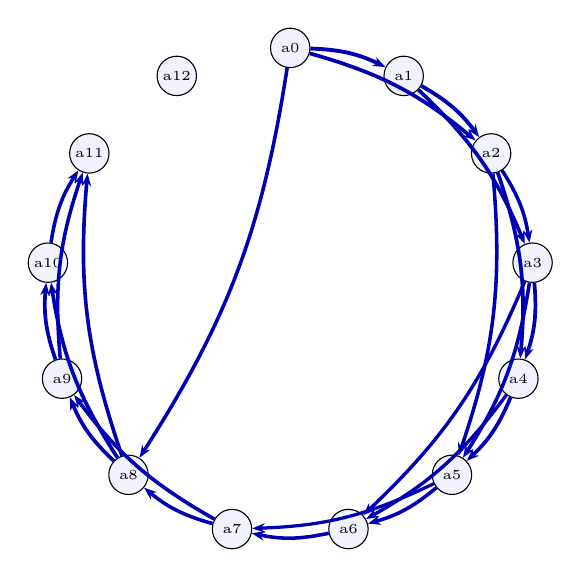
\begin{tikzpicture}[>={Stealth[length=1.6mm]}]
  \node[circle,draw,fill=blue!5,inner sep=1pt,minimum size=5mm,font=\tiny] (a0) at (90.0:3.10) {a0};
  \node[circle,draw,fill=blue!5,inner sep=1pt,minimum size=5mm,font=\tiny] (a1) at (62.3:3.10) {a1};
  \node[circle,draw,fill=blue!5,inner sep=1pt,minimum size=5mm,font=\tiny] (a2) at (34.6:3.10) {a2};
  \node[circle,draw,fill=blue!5,inner sep=1pt,minimum size=5mm,font=\tiny] (a3) at (6.9:3.10) {a3};
  \node[circle,draw,fill=blue!5,inner sep=1pt,minimum size=5mm,font=\tiny] (a4) at (-20.8:3.10) {a4};
  \node[circle,draw,fill=blue!5,inner sep=1pt,minimum size=5mm,font=\tiny] (a5) at (-48.5:3.10) {a5};
  \node[circle,draw,fill=blue!5,inner sep=1pt,minimum size=5mm,font=\tiny] (a6) at (-76.2:3.10) {a6};
  \node[circle,draw,fill=blue!5,inner sep=1pt,minimum size=5mm,font=\tiny] (a7) at (-103.8:3.10) {a7};
  \node[circle,draw,fill=blue!5,inner sep=1pt,minimum size=5mm,font=\tiny] (a8) at (-131.5:3.10) {a8};
  \node[circle,draw,fill=blue!5,inner sep=1pt,minimum size=5mm,font=\tiny] (a9) at (-159.2:3.10) {a9};
  \node[circle,draw,fill=blue!5,inner sep=1pt,minimum size=5mm,font=\tiny] (a10) at (-186.9:3.10) {a10};
  \node[circle,draw,fill=blue!5,inner sep=1pt,minimum size=5mm,font=\tiny] (a11) at (-214.6:3.10) {a11};
  \node[circle,draw,fill=blue!5,inner sep=1pt,minimum size=5mm,font=\tiny] (a12) at (-242.3:3.10) {a12};
  \draw[-{Stealth[length=1.6mm]}, blue!70!black, line width=1.40pt] (a0) to[bend left=12] (a1);
  \draw[-{Stealth[length=1.6mm]}, blue!70!black, line width=1.34pt] (a0) to[bend left=12] (a2);
  \draw[-{Stealth[length=1.6mm]}, blue!70!black, line width=1.38pt] (a1) to[bend left=12] (a2);
  \draw[-{Stealth[length=1.6mm]}, blue!70!black, line width=1.34pt] (a1) to[bend left=12] (a3);
  \draw[-{Stealth[length=1.6mm]}, blue!70!black, line width=1.28pt] (a2) to[bend left=12] (a3);
  \draw[-{Stealth[length=1.6mm]}, blue!70!black, line width=1.34pt] (a2) to[bend left=12] (a4);
  \draw[-{Stealth[length=1.6mm]}, blue!70!black, line width=1.28pt] (a2) to[bend left=12] (a5);
  \draw[-{Stealth[length=1.6mm]}, blue!70!black, line width=1.34pt] (a3) to[bend left=12] (a4);
  \draw[-{Stealth[length=1.6mm]}, blue!70!black, line width=1.28pt] (a3) to[bend left=12] (a5);
  \draw[-{Stealth[length=1.6mm]}, blue!70!black, line width=1.23pt] (a3) to[bend left=12] (a6);
  \draw[-{Stealth[length=1.6mm]}, blue!70!black, line width=1.34pt] (a4) to[bend left=12] (a5);
  \draw[-{Stealth[length=1.6mm]}, blue!70!black, line width=1.23pt] (a4) to[bend left=12] (a6);
  \draw[-{Stealth[length=1.6mm]}, blue!70!black, line width=1.28pt] (a5) to[bend left=12] (a6);
  \draw[-{Stealth[length=1.6mm]}, blue!70!black, line width=1.17pt] (a5) to[bend left=12] (a7);
  \draw[-{Stealth[length=1.6mm]}, blue!70!black, line width=1.28pt] (a6) to[bend left=12] (a7);
  \draw[-{Stealth[length=1.6mm]}, blue!70!black, line width=1.28pt] (a7) to[bend left=12] (a8);
  \draw[-{Stealth[length=1.6mm]}, blue!70!black, line width=1.31pt] (a7) to[bend left=12] (a9);
  \draw[-{Stealth[length=1.6mm]}, blue!70!black, line width=1.34pt] (a8) to[bend left=12] (a9);
  \draw[-{Stealth[length=1.6mm]}, blue!70!black, line width=1.34pt] (a8) to[bend left=12] (a10);
  \draw[-{Stealth[length=1.6mm]}, blue!70!black, line width=1.31pt] (a8) to[bend left=12] (a11);
  \draw[-{Stealth[length=1.6mm]}, blue!70!black, line width=1.34pt] (a9) to[bend left=12] (a10);
  \draw[-{Stealth[length=1.6mm]}, blue!70!black, line width=1.28pt] (a9) to[bend left=12] (a11);
  \draw[-{Stealth[length=1.6mm]}, blue!70!black, line width=1.28pt] (a10) to[bend left=12] (a11);
  \draw[-{Stealth[length=1.6mm]}, blue!70!black, line width=1.28pt] (a0) to[bend left=12] (a8);
\end{tikzpicture}
}
\\[2pt]{\footnotesize gate: 24 relations}
\end{minipage}
\caption{Relation graph for \texttt{ex6-incident} (Software incident post-mortem (coherent)): gate.}
\label{fig:graph-example-6-incident}
\end{figure}

\section{Conclusion}

The experiment harness runs the full LCS pipeline end to end --- atom-pair
relation mining, coherence Markov-random-field construction, and all four score
readouts (mean marginal support, consistency probability, reified coherence node,
and normalized log-partition) --- across multiple models and conditional-strength
uncertainty-quantification methods. Three findings are robust. First, the choice
of conditional-strength UQ method (surrogate-token from logprobs, sampled affirm
fraction, or the verbalized baseline) materially changes the mined edge weights
and therefore the LCS, confirming that the strength estimator is a first-class
design decision rather than a detail. Second, the four readouts agree on the
ordering of coherent versus contradiction-bearing responses but differ in dynamic
range, so the headline mean-marginal score is best reported alongside the
log-partition diagnostic. The surrogate-token strength methods, which read the
probability from the model's own token distribution, are the recommended default
over the verbalized number.

Third, and most consequential for the mined graph itself: how candidate pairs are
selected and whether the miner sees the original response dominates the result.
Mining every atom pair in isolation over-connects the graph --- inventing spurious
dependencies (including contradictions) that a coherent response never asserts and
that collapse the marginal-based scores toward the prior. Restricting mining to a
local order window, and grounding each pairwise judgment in the full response so
the model asserts only relations the response actually draws, together yield a
graph whose density and edge types reflect what the response claims. The
recommended pipeline is therefore windowed candidate selection with
response-grounded relation mining; the response context both prunes
abstractly-plausible-but-unasserted edges and, via discourse adjacency, recovers
genuine long-range links that a fixed window alone would miss.

\section{Future work}

Several directions follow naturally.
\begin{itemize}
  \item \textbf{Calibration on labeled relations.} Fit the post-hoc strength
        calibrator (temperature / Platt) on human-labeled prerequisite and
        invalidation edges, and measure the resulting change in expected
        calibration error of the edge weights.
  \item \textbf{Larger model and method sweep.} Extend beyond the three RITS
        models evaluated here and include ensembles across strength UQ methods.
  \item \textbf{Human-rated coherence correlation.} Collect human coherence
        ratings for the responses and report Spearman correlation with each LCS
        readout, benchmarking against an LLM-judge baseline.
  \item \textbf{Validating grounded recall on long responses.} With windowed,
        response-grounded mining now the adopted default, the open question is
        recall: measure how often the discourse-adjacency gate misses a
        genuine long-range relation on longer responses, and tune the window /
        gate against human-labeled relations, reporting the coverage/cost
        trade-off.
  \item \textbf{Joint factuality and coherence.} Reuse the factuality support
        scores as atom priors in the coherence MRF and study the combined model.
\end{itemize}

\end{document}
